% Options for packages loaded elsewhere
\PassOptionsToPackage{unicode}{hyperref}
\PassOptionsToPackage{hyphens}{url}
\PassOptionsToPackage{dvipsnames,svgnames,x11names}{xcolor}
\documentclass[
  10pt,
  fontset=fandol]{ctexart}
\usepackage{xcolor}
\usepackage[margin=16mm]{geometry}
\usepackage{amsmath,amssymb}
\setcounter{secnumdepth}{-\maxdimen} % remove section numbering
\usepackage{iftex}
\ifPDFTeX
  \usepackage[T1]{fontenc}
  \usepackage[utf8]{inputenc}
  \usepackage{textcomp} % provide euro and other symbols
\else % if luatex or xetex
  \usepackage{unicode-math} % this also loads fontspec
  \defaultfontfeatures{Scale=MatchLowercase}
  \defaultfontfeatures[\rmfamily]{Ligatures=TeX,Scale=1}
\fi
\usepackage{lmodern}
\ifPDFTeX\else
  % xetex/luatex font selection
\fi
% Use upquote if available, for straight quotes in verbatim environments
\IfFileExists{upquote.sty}{\usepackage{upquote}}{}
\IfFileExists{microtype.sty}{% use microtype if available
  \usepackage[]{microtype}
  \UseMicrotypeSet[protrusion]{basicmath} % disable protrusion for tt fonts
}{}
\makeatletter
\@ifundefined{KOMAClassName}{% if non-KOMA class
  \IfFileExists{parskip.sty}{%
    \usepackage{parskip}
  }{% else
    \setlength{\parindent}{0pt}
    \setlength{\parskip}{6pt plus 2pt minus 1pt}}
}{% if KOMA class
  \KOMAoptions{parskip=half}}
\makeatother
\usepackage{graphicx}
\makeatletter
\newsavebox\pandoc@box
\newcommand*\pandocbounded[1]{% scales image to fit in text height/width
  \sbox\pandoc@box{#1}%
  \Gscale@div\@tempa{\textheight}{\dimexpr\ht\pandoc@box+\dp\pandoc@box\relax}%
  \Gscale@div\@tempb{\linewidth}{\wd\pandoc@box}%
  \ifdim\@tempb\p@<\@tempa\p@\let\@tempa\@tempb\fi% select the smaller of both
  \ifdim\@tempa\p@<\p@\scalebox{\@tempa}{\usebox\pandoc@box}%
  \else\usebox{\pandoc@box}%
  \fi%
}
% Set default figure placement to htbp
\def\fps@figure{htbp}
\makeatother
\setlength{\emergencystretch}{3em} % prevent overfull lines
\providecommand{\tightlist}{%
  \setlength{\itemsep}{0pt}\setlength{\parskip}{0pt}}
\usepackage{amsmath,amssymb,mathtools,needspace}
\xeCJKDeclareCharClass{CJK}{"2032,"0400->"04FF,"2160->"216B,"2460->"2473,"25A0,"25C7,"25CB,"25CF}
\IfFontExistsTF{Arial Unicode MS}{\xeCJKsetup{AutoFallBack=true}\setCJKfallbackfamilyfont{\CJKrmdefault}{Arial Unicode MS}}{}
\setcounter{secnumdepth}{0}
\setlength{\emergencystretch}{2em}
\allowdisplaybreaks
\usepackage{bookmark}
\IfFileExists{xurl.sty}{\usepackage{xurl}}{} % add URL line breaks if available
\urlstyle{same}
\hypersetup{
  pdftitle={Walsh函数的复杂性},
  colorlinks=true,
  linkcolor={Maroon},
  filecolor={Maroon},
  citecolor={Blue},
  urlcolor={Blue},
  pdfcreator={LaTeX via pandoc}}

\title{Walsh函数的复杂性}
\author{}
\date{}

\begin{document}
\maketitle

\subsubsection{10.1.2　Walsh 函数的复杂性}\label{walsh-ux51fdux6570ux7684ux590dux6742ux6027}

1923 年，美国数学家 J. L. Walsh 又提出了一个完备的正交函数系，后人将其称作 Walsh 函数系。第 \(k\) 族 Walsh 函数含有 \(2^k\) 个函数，其中第 \(i\) 个函数 \(W_{ki}\) 有如下解析表达式：

\[
\begin{gathered}
W_{ki}(x)=\prod_{r=0}^{k-1}\operatorname{sgn}[\cos i_r2^r\pi x],\quad 0\leqslant x<1,\\
k=0,1,2,\cdots,\quad i=0,1,\cdots,2^k-1,
\end{gathered}
\]

式中，\(\operatorname{sgn}\) 是\textbf{符号函数}，当 \(x\geqslant0\) 时 \(\operatorname{sgn}[x]\) 取值 \(+1\)，而 \(x<0\) 时取值 \(-1\)。又 \(i_r\) 取值 \(0\) 或 \(1\) 是序数 \(i\) 的二进制码：

\[
i=\sum_{r=0}^{k-1}i_r2^r.
\]

图 10.1 列出前面 16 个 Walsh 函数的波形。其中，第 1 个（标号 0）组成第 0 族，前两个（标号 0 与 1）组成第 1 族；前 4 个（标号 0、1、2、3）组成第 2 族，依此类推，前 16 个组成第 4 族 Walsh 函数。

Walsh 函数取值简单，它们仅取 \(\pm1\) 两个值，但其波形却很复杂，似乎比三角函数要复杂得多，以致依据定义很难作出它们的图形。

由于表达式中含有符号运算 \(\operatorname{sgn}\)，Walsh 函数的波形频繁起伏，甚至``几乎处处''不连续（见图 10.1），经典的微积分方法在这里难以施展身手，Walsh 函数系的形态

\href{../../source-images/pdf-263.jpeg}{原页}

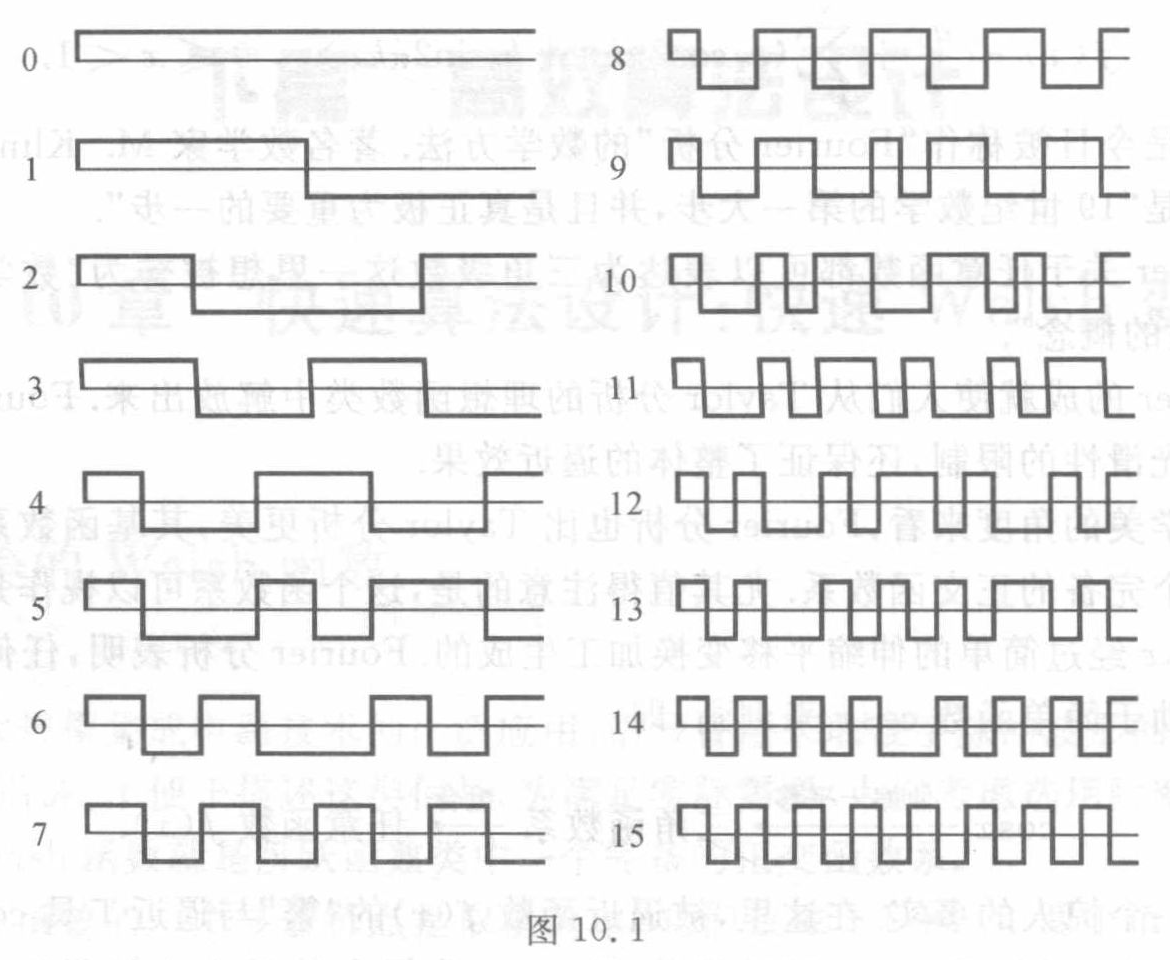
\includegraphics[width=0.85\linewidth,height=\textheight,keepaspectratio,alt={图 10.1（原图裁切）：前 16 个 Walsh 函数的波形}]{../assets/ch10/fig-10-1.png}

图 10.1

\begin{quote}
图中文字与图意（转录）：左列波形标号依次为 0、1、2、3、4、5、6、7，右列依次为 8、9、10、11、12、13、14、15。各条波形在水平基线上下取两个阶跃值；标号 0 的波形为方波。
\end{quote}

怪异与表达式复杂使人们对它望而却步，在提出后的许多年里，它一直默默无闻，不被人们所重视。

直到 20 世纪 60 年代末，人们才惊异地发现，Walsh 函数可应用于信号处理的众多领域，诸如通信、声呐、雷达、图像处理、语音识别、遥感遥测遥控、仪表、医学、天文、地质等等。

``真''是``美''的反光。有着广泛应用的 Walsh 函数美在哪里呢？

\end{document}
